\subsection{System Architecture and Data Model}

This section presents different architectural perspectives of the LiftDrop system, including component-level interactions and data model relationships. Each view emphasizes a specific aspect of the system's behavior, from geolocation handling to user roles and delivery lifecycle.

\subsubsection{High-Level System Architecture}

Figure~\ref{fig:high-level-Overview} illustrates the top-level architecture of the LiftDrop platform. It shows how the Android mobile application communicates with backend services responsible for order management, user interaction, real-time communication, and location processing.

\vspace{8mm}

\begin{figure}[H]
    \centering
    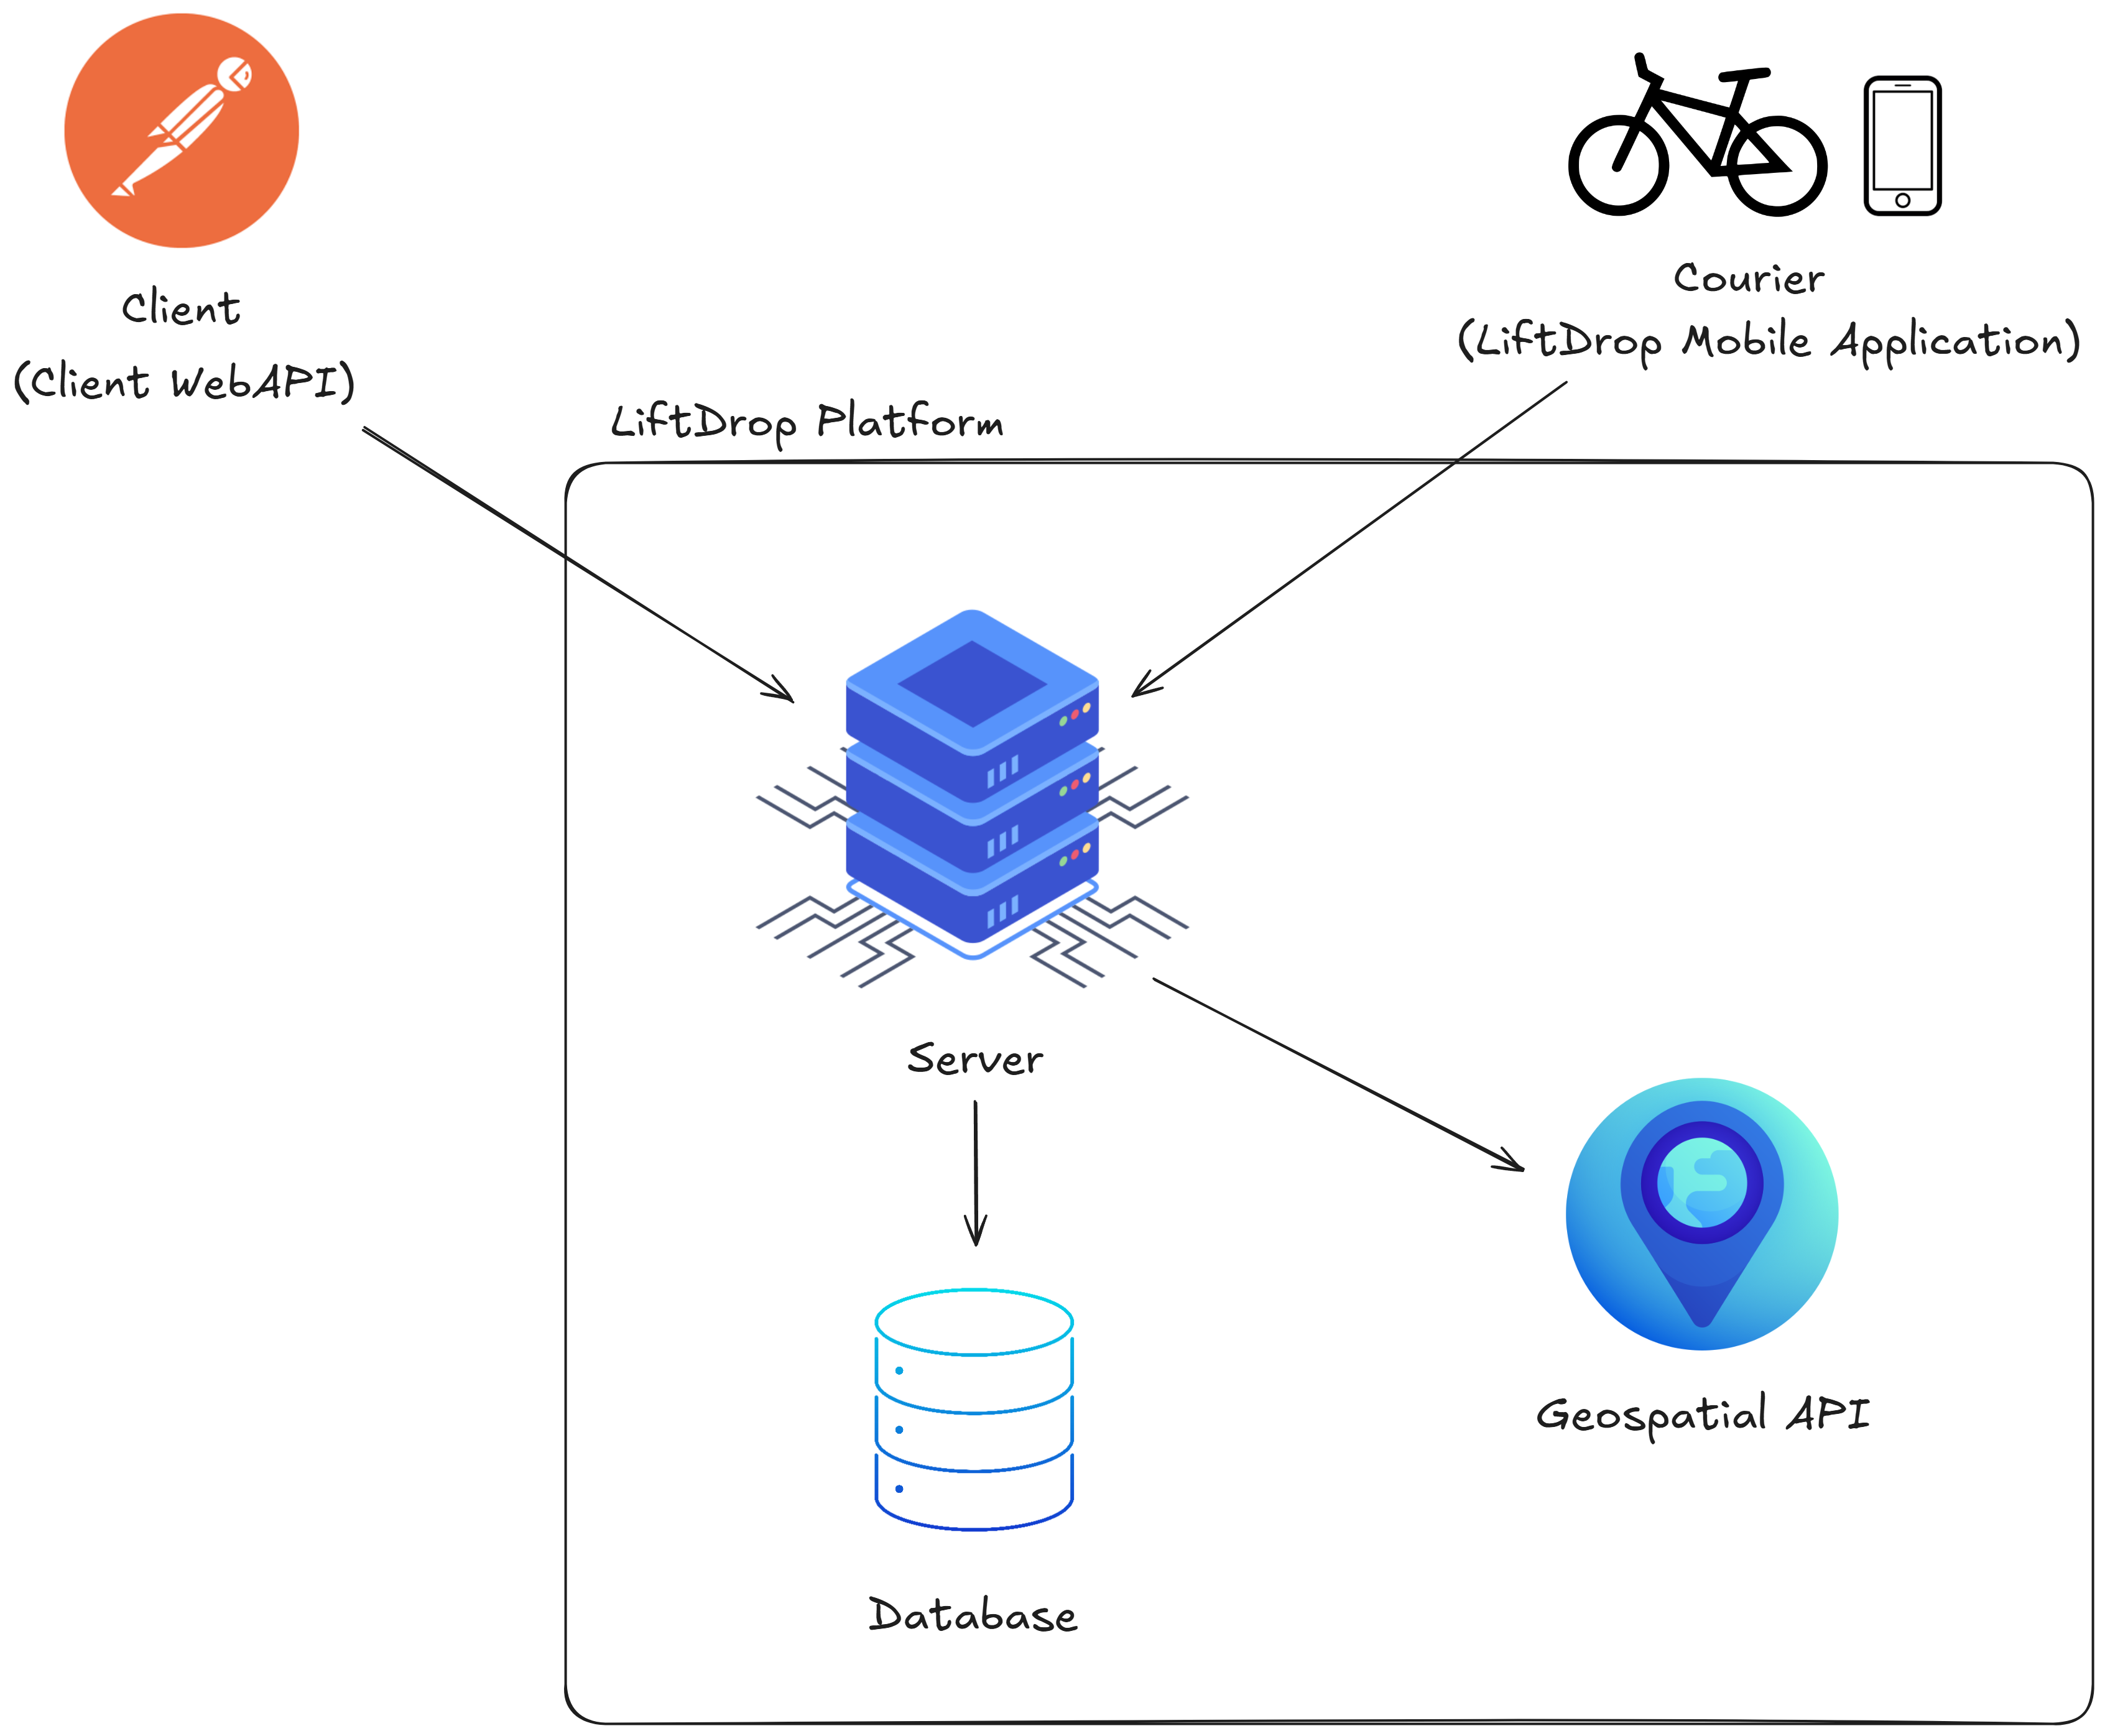
\includegraphics[width=0.82\textwidth]{images/LiftDrop_High_level_view.png}
    \caption{High-level overview of the LiftDrop system architecture}
    \label{fig:high-level-Overview}
\end{figure}

\newpage

\subsubsection{Location Model Overview}

This view isolates the system's handling of geospatial information. The \texttt{Location} class acts as a base abstraction for different types of spots used during a delivery. Specialized entities like \texttt{PickupSpot} and \texttt{DropOffSpot} inherit from \texttt{Location}, allowing consistent treatment of position data. A pickup spot can contain multiple \texttt{Item} entries, each identified by a unique designation.

\begin{figure}[H]
    \centering
    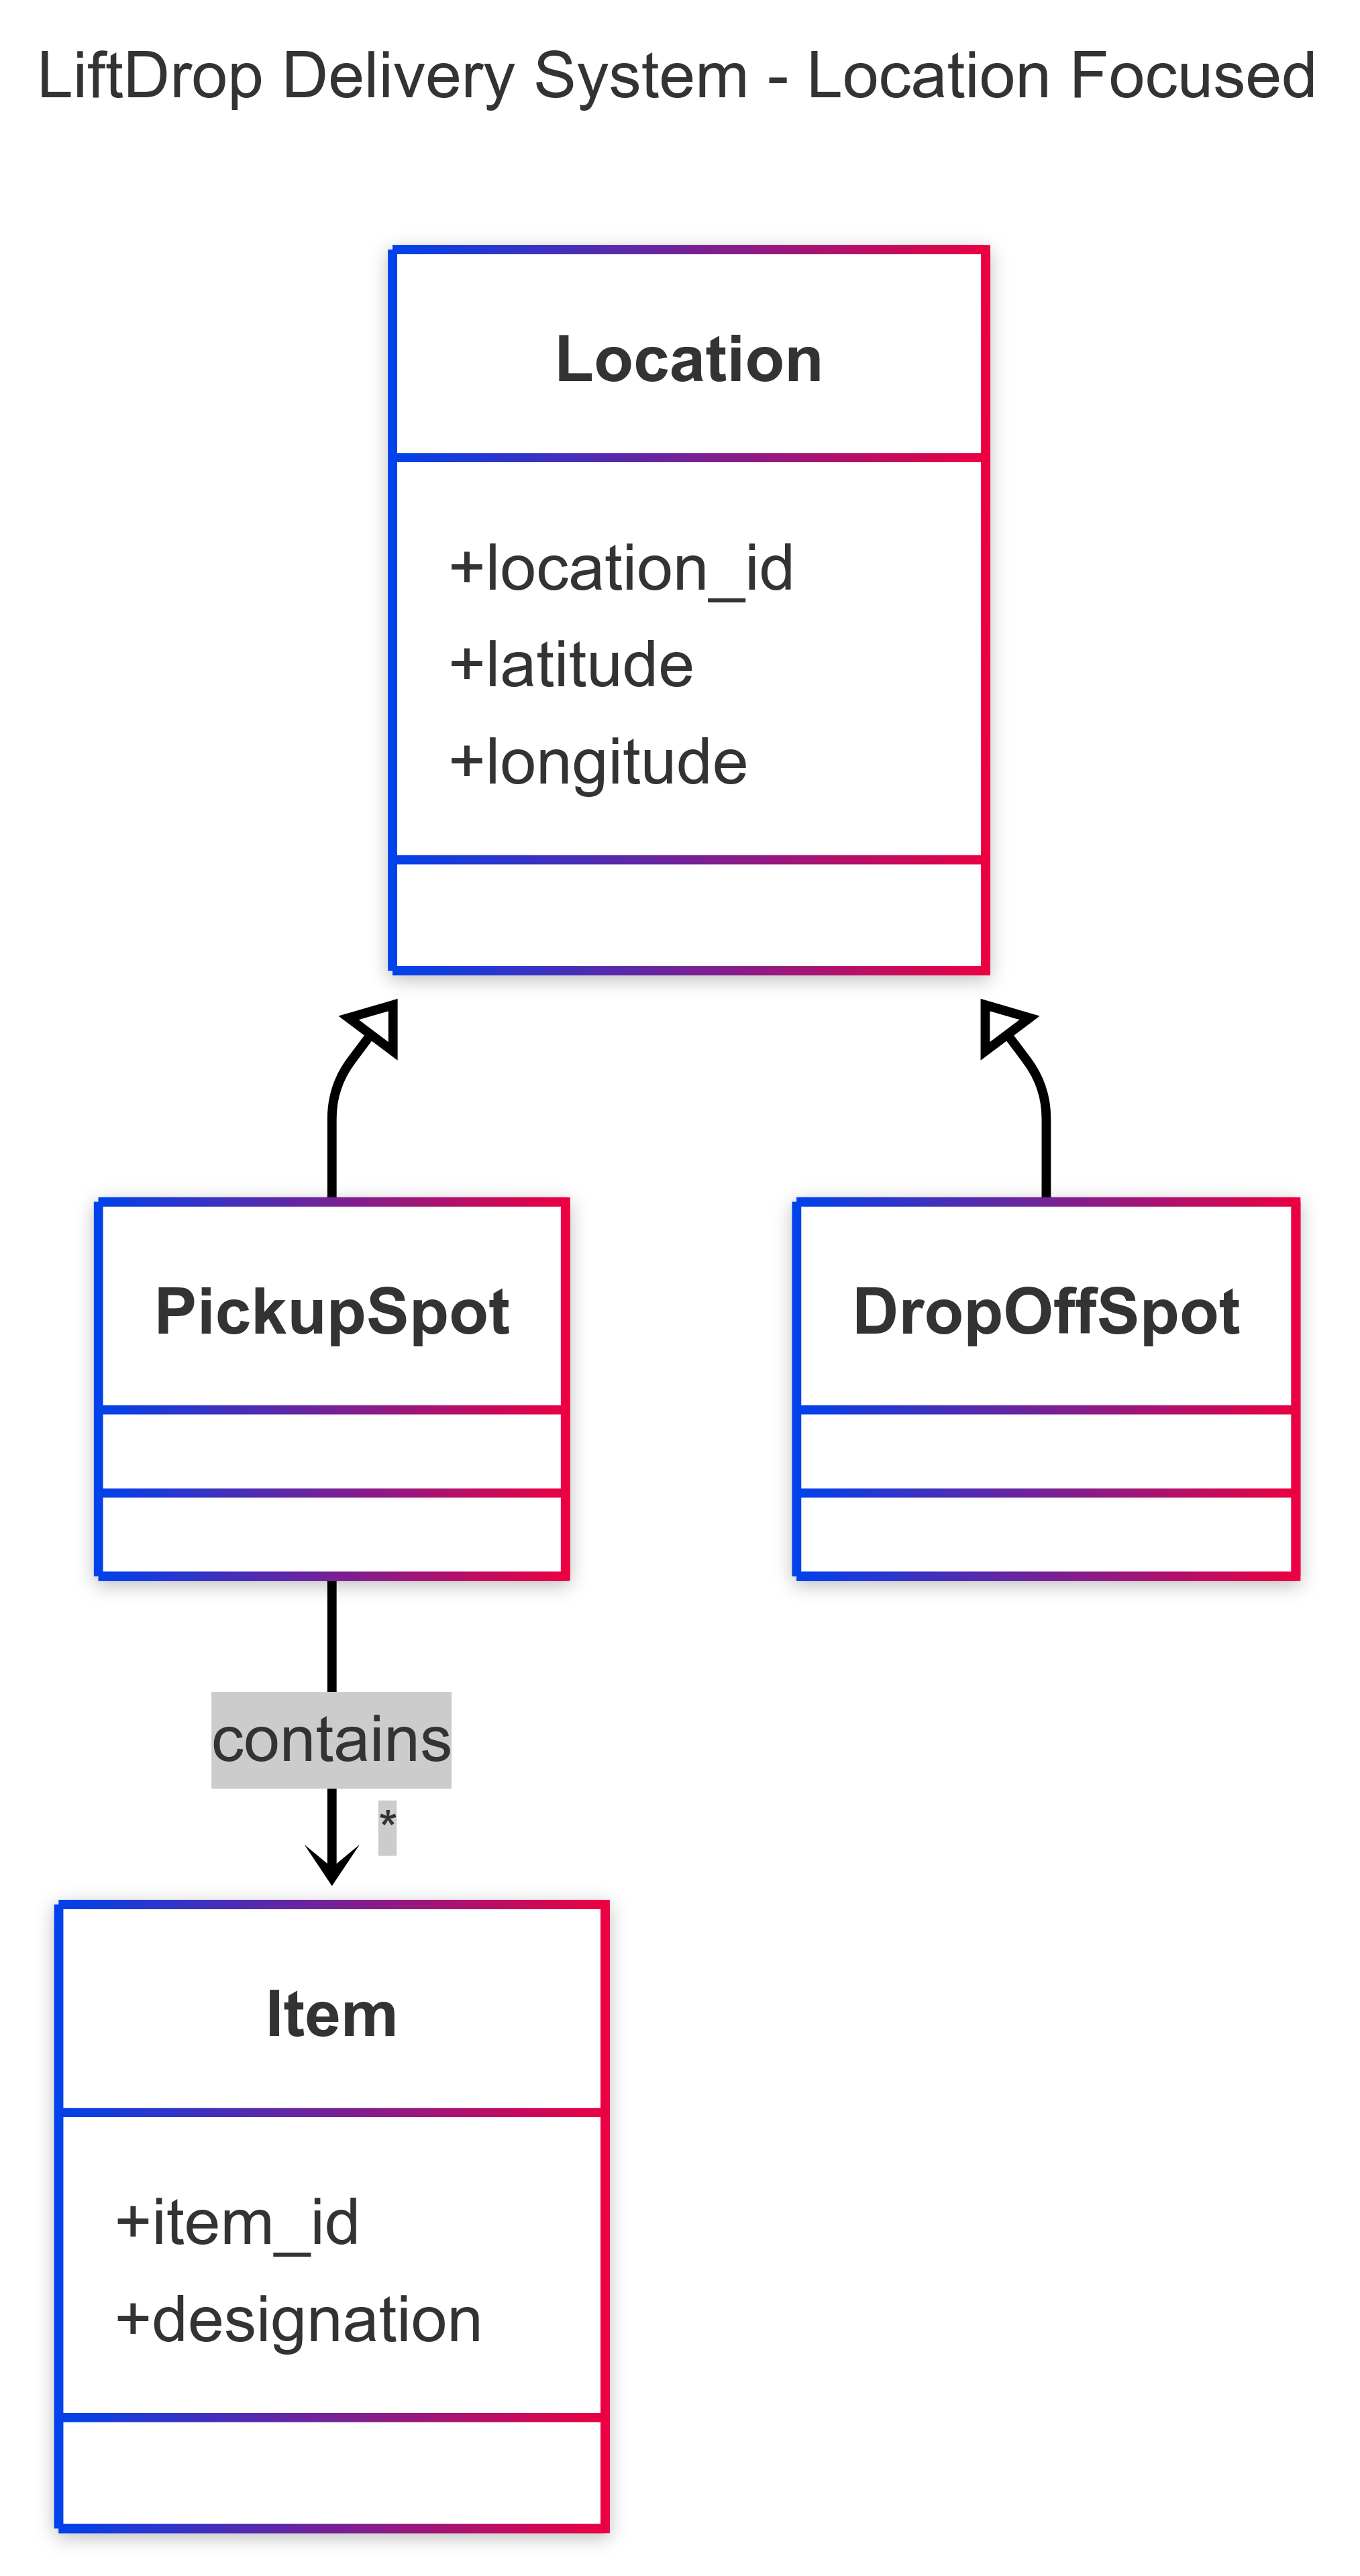
\includegraphics[width=0.44\textwidth]{images/LocationDiagram.png}
    \caption{Location Model Structure}
\end{figure}

\newpage

\subsubsection{User Role and Interaction Model}

This simplified diagram captures user roles and their interaction with delivery workflows. A \texttt{Client} can place multiple \texttt{Request}s, and a \texttt{Courier} can fulfill many of them. Each request is linked to a corresponding \texttt{Delivery}, forming a one-to-one mapping between a request and its fulfillment.
  
\begin{figure}[H]
    \centering
    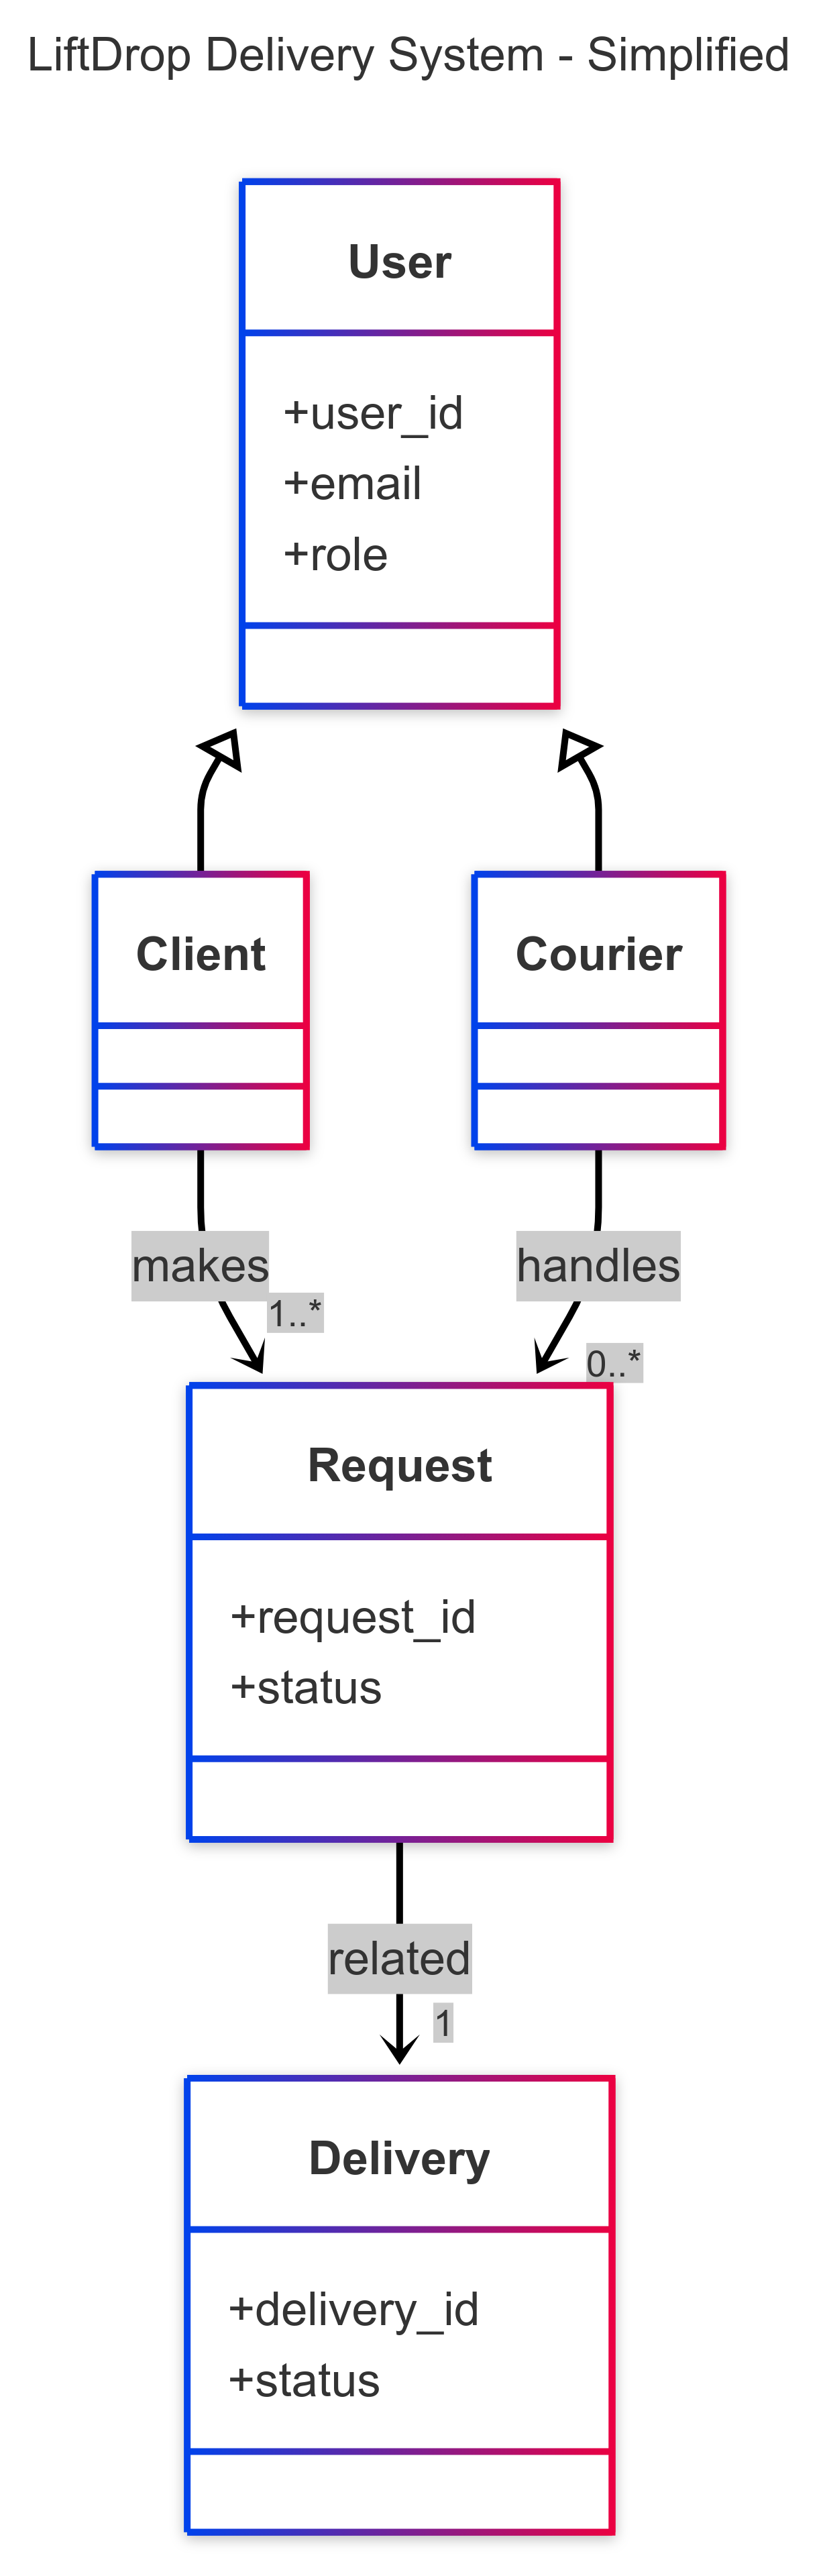
\includegraphics[width=0.40\textwidth]{images/UserClientCourierDiagram.png}
    \caption{User and Role Relationships}
\end{figure}

\subsubsection{Request and Delivery Lifecycle View}

This view focuses on how a request progresses through the system. Each \texttt{Request} includes additional metadata encapsulated in a \texttt{RequestDetails} object and is associated with a single \texttt{Delivery}. This structure supports clear traceability and separation of concerns between request creation and execution.

\begin{figure}[H]
    \centering
    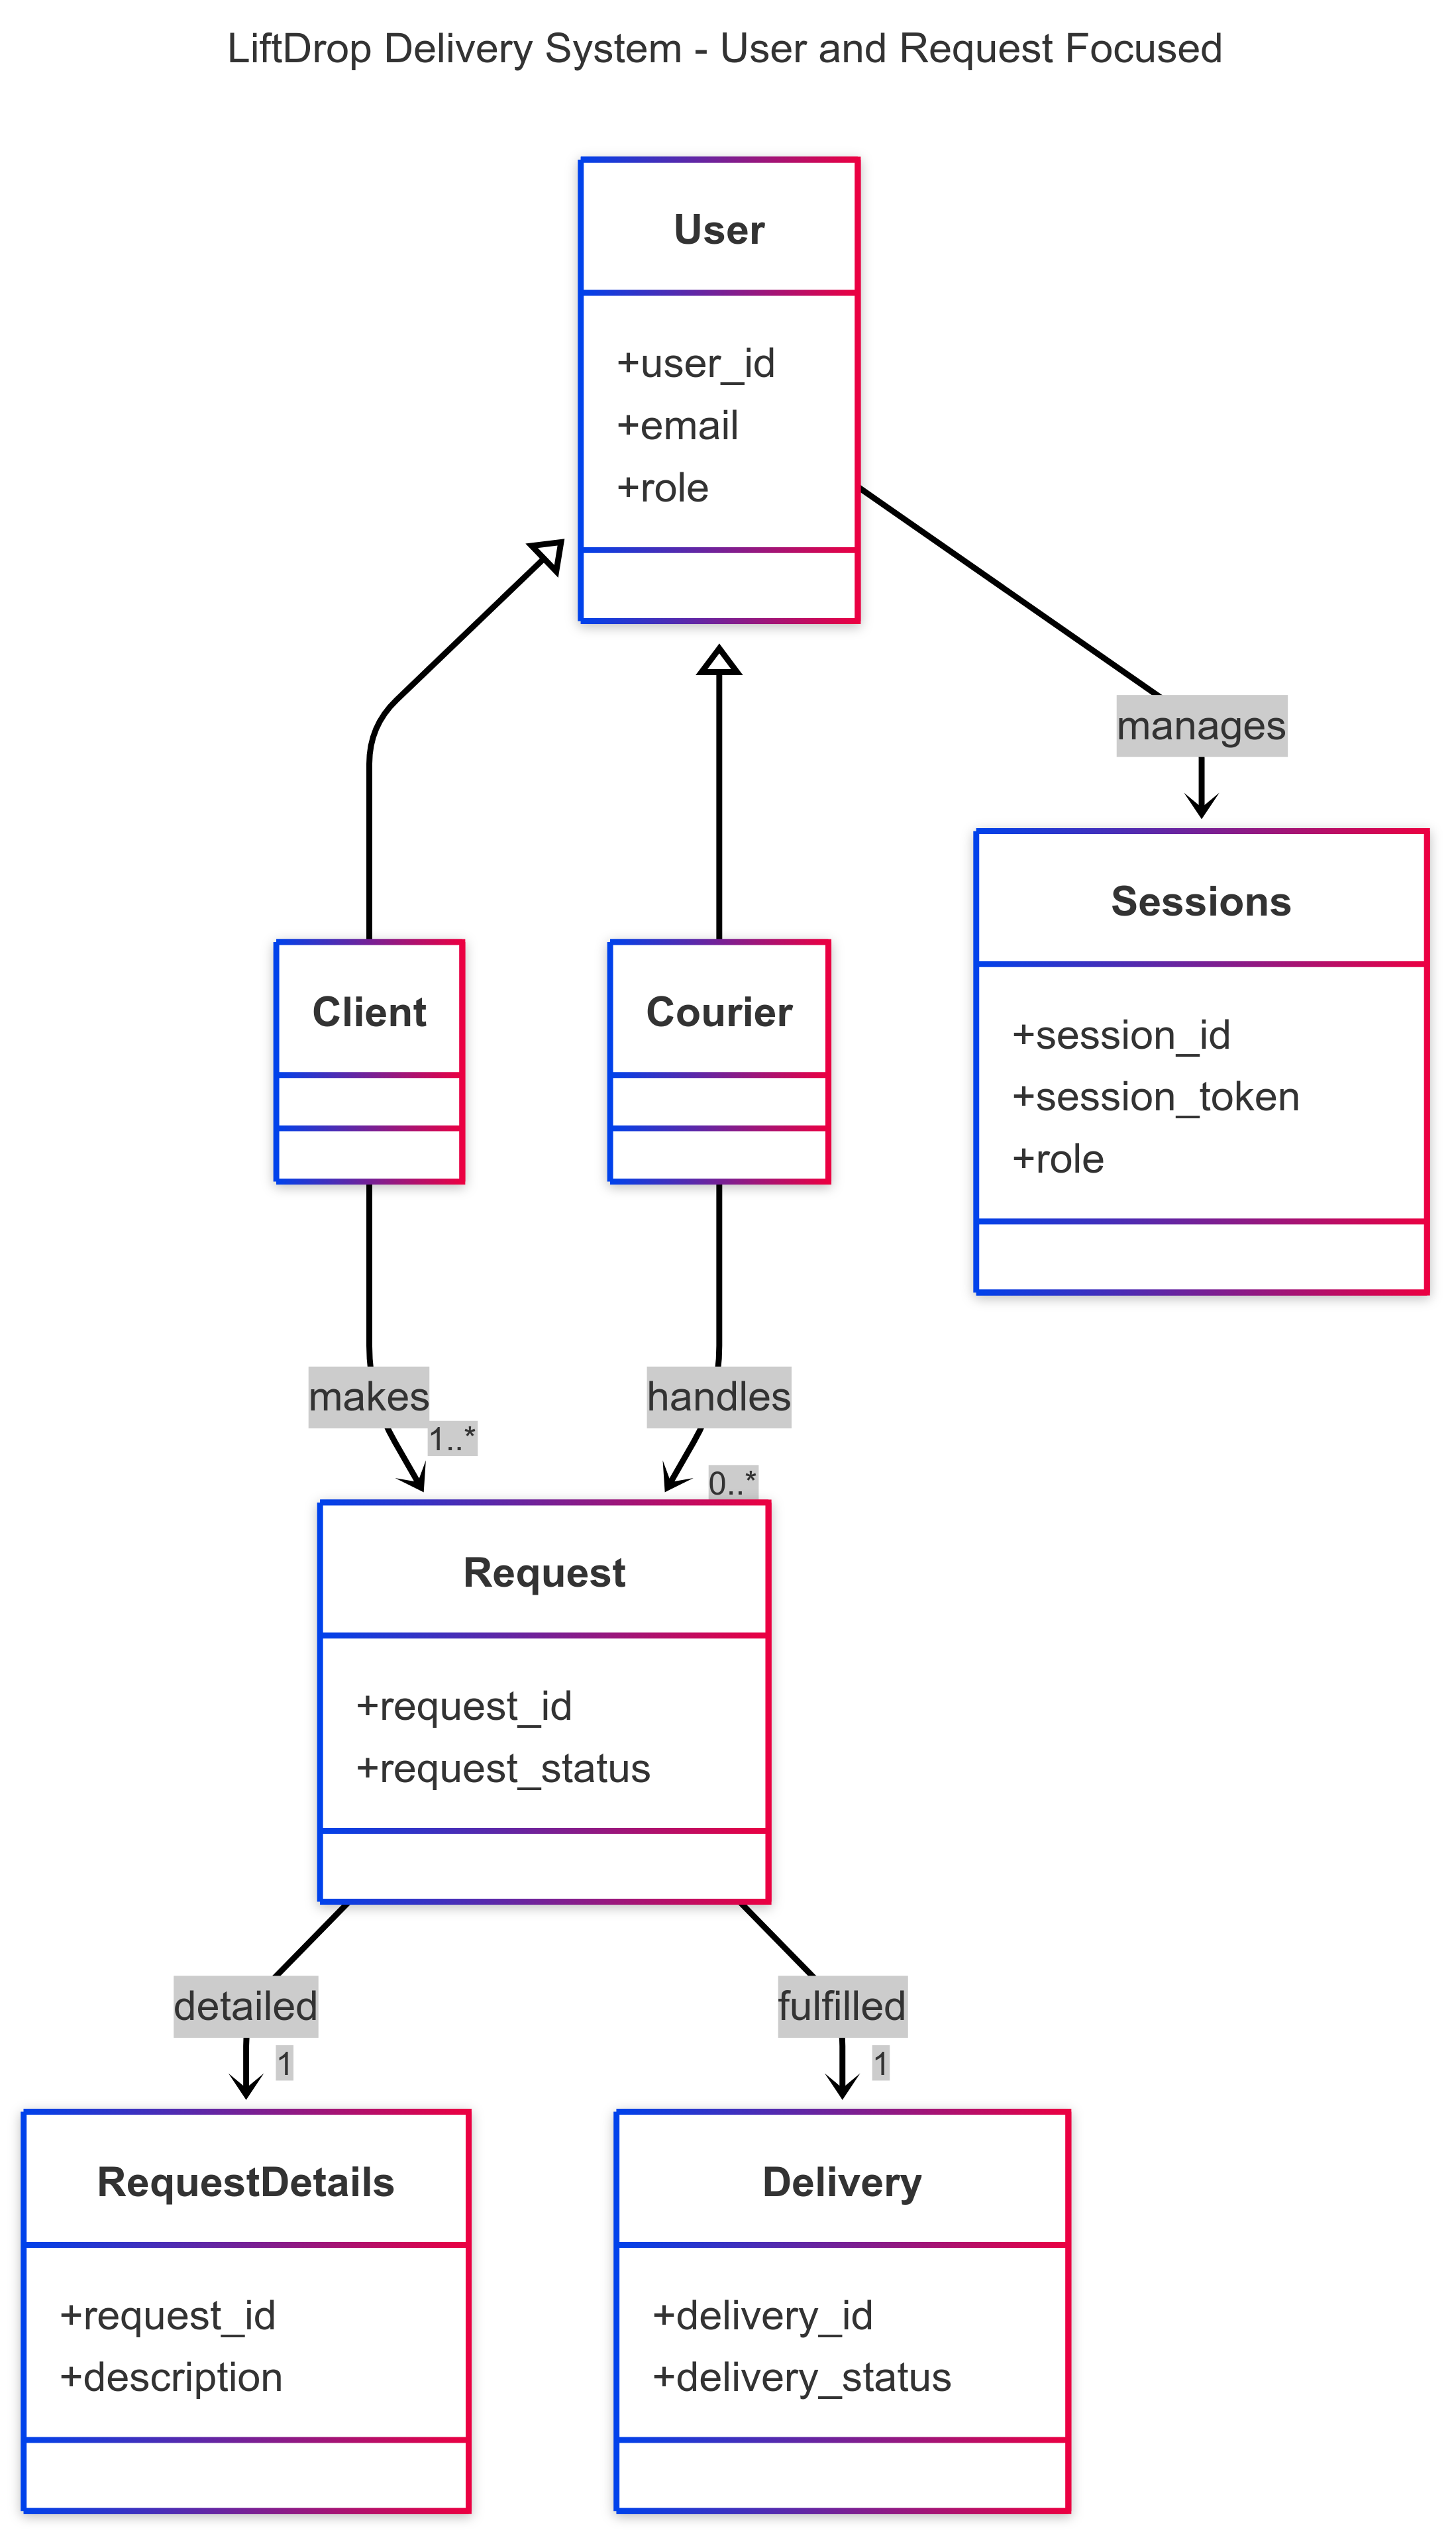
\includegraphics[width=0.44\textwidth]{images/UserSessions.png}
    \caption{Request and Fulfillment Architecture}
\end{figure}

\newpage

\subsubsection{Comprehensive System Model}

The complete data model integrates all key domain entities: \texttt{User}, \texttt{Address}, \texttt{Location}, \texttt{Item}, \texttt{Request}, \texttt{Delivery}, and \texttt{Session}. It captures how users interact with the system, how orders are structured and routed, and how real-time delivery coordination is maintained through geolocation and session-aware tracking.

\begin{figure}[H]
    \centering
    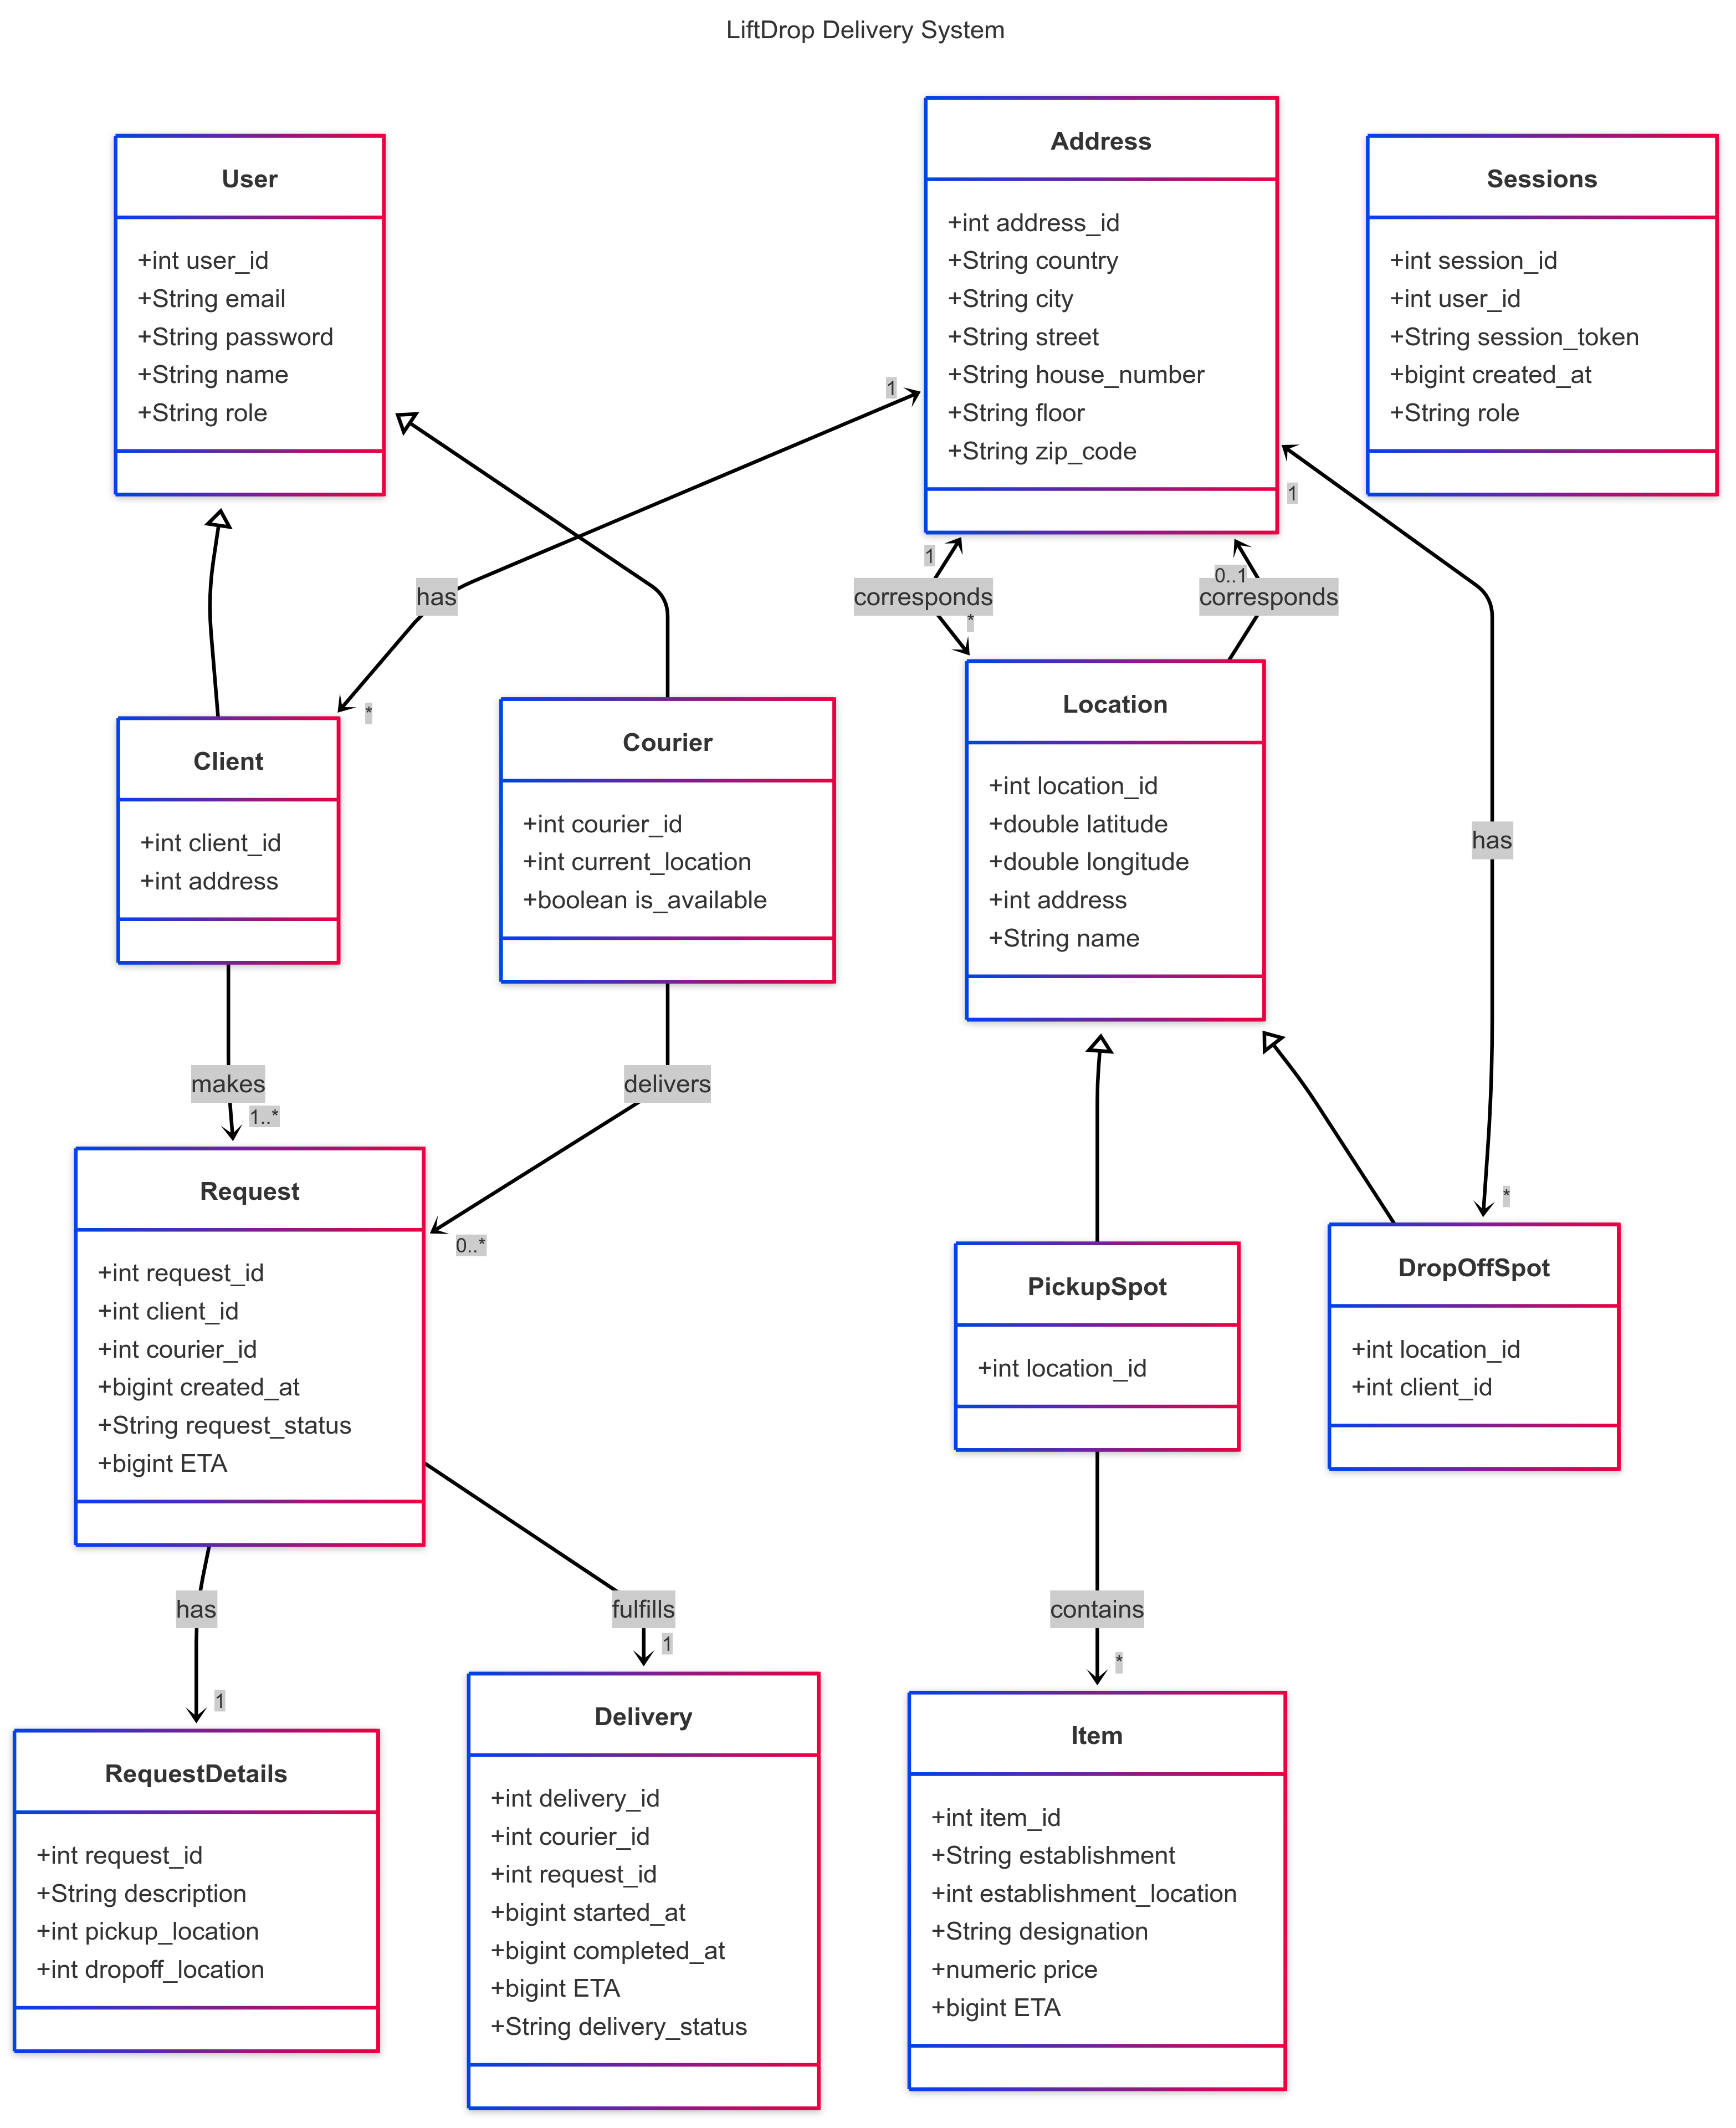
\includegraphics[width=0.8\textwidth]{images/FullDiagram.png}
    \caption{Full System Data Model}
\end{figure}
